
\section{Deep learning approaches for time series classification}
\label{appendix:2}

As already mentioned Step scan dataset, with the nature of video-based, is the data set that we used in this research. It should be noted that this type of dataset is basically suitable for this project and there is no need to convert the image into a time-series signal, however since our goal in this research is developing machine learning models from the time-series dataset, so we turned the video data set into a time-series one in order to implement a variety of classic machine learning algorithms and also deep learning methods, named LDA, KNN, SVM and Random forest which are categorized in machine learning algorithms and CNN, inception time and Echo State as deep learning methods. Therefore, in this appendix, we have tried to give a brief explanation of time series classification and main deep learning methods.


\subsection{Introduction}

It has been for two decades that time series classification has been regarded as one of the most challenging problems in data mining \cite{Esling2012Time-seriesMining}. Any classification problem which uses data taking into account some indication of order can be accounted as a Time series classification (TSC) case \cite{Gamboa2017DeepAnalysis}.  The field of computer has been seen as a big bang, once a Deep Convolutional Neural network has been proposed \cite{Krizhevsky2017ImageNetNetworks}. These algorithms deep learning models could handle feature engineering automatically and internally, they optimize and eradicate it without the need of doing it manually. This caused many applications in many different domains utilize these networks.  


\subsection{Deep learning}

Figure \ref{fig:a1} shows a general Deep Learning framework for time series classification. It is a composition of several layers that implement non-linear functions. The input could be eighter a multivariate time series or univariate data. Every layer takes as input the output of the previous layer and applies its non-linear transformation to compute its own output.
In this research, 5 different Deep Learning architectures for time series classifications are presented. 



\begin{figure}[H]
    \centering
    \begin{minipage}[b]{\textwidth}
        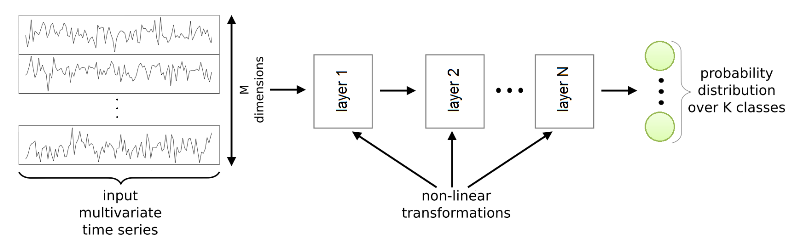
\includegraphics[width=\textwidth]{figures/project/app1.png}
    \end{minipage}
    \caption{The general Deep Learning framework for time series classification.}
    \label{fig:a1}
\end{figure}

\subsection{Convolutional Neural Networks}

Since AlexNet \cite{Krizhevsky2017ImageNetNetworks} won the imageNet competition in 2012, deep CNNs have seen a lot of successful applications in many different domains such as reaching human-level performance in image recognition problems as well as different natural language processing tasks. Motivated by the success of these CNN architectures in these various domains, researchers have started adopting them for time series analysis \cite{Gamboa2017DeepAnalysis}. 

The challenges of using this architecture is changing time series data to image data. Some papers used several techniques like Continuous Wavelet Transform (CWT) \cite{Wang2021AutomaticNetwork}, Recurrence Plots (RP) \cite{Hatami2017ClassificationNetworks}, and short-time Fourier transform (STFT) \cite{Huang2019ECGNetwork} to produce a 2D representation of time-series and therefore time series classification can change to a texture image recognition task.

Weng et al. in \cite{WangTimeBaseline} used a 1D convolutional operation to adapt this architecture to time series data. They tested three deep neural network architectures, MLP, FCN and Residual Network, to provide a comprehensive baseline model in time series.




\subsection{Inception Time}
Recently a deep Convolutional Neural Network called Inception Time was introduced by Fawaz et al. in \cite{IsmailFawaz2020InceptionTime:Classification}. This kind of network shows high accuracy and scalability. As shown in the figure \ref{fig:a2}, the Inception Network consists of a series of Inception Modules followed by a Global Average Pooling Layer and a Fully Connected Layer (usually a Multi-Layer Perceptron). Moreover, a residual connection is added at every third inception module. Each residual block’s input is transferred via a shortcut linear connection to be added to the next block’s input, thus mitigating the vanishing gradient problem by allowing a direct flow of the gradient.

\begin{figure}[H]
    \centering
    \begin{minipage}[b]{\textwidth}
        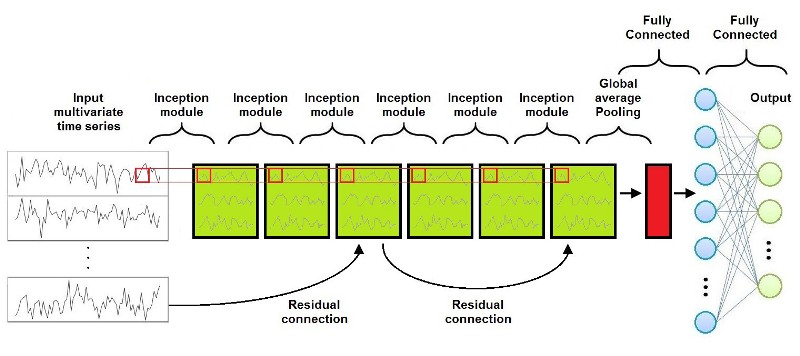
\includegraphics[width=\textwidth]{manuscript/src/figures/project/app2.jpeg}
    \end{minipage}
    \caption{Inception Network Architecture \cite{IsmailFawaz2020InceptionTime:Classification}}
    \label{fig:a2}
\end{figure}


\subsection{Echo State Networks}

Echo State Networks \cite{Bianchi2018ReservoirSeries} are a type of Recurrent Neural Network. Hence it can be useful to have a small introduction about them. Recurrent Neural Networks are networks of neuron-like nodes organized into successive layers, with an architecture similar to one of the standard Neural Networks. In fact, like in standard Neural Networks, neurons are divided into the input layer, hidden layers and output layers. Each connection between neurons has a corresponding trainable weight.  

As has shown in the figure \ref{fig:a3} , the architecture of an Echo State Network consists of an Input Layer, a hidden Layer called Reservoir, a Dimension Reduction Layer, a Fully Connected Layer called Readout, and an Output Layer.

In general, the main difficulty in using CNNs is that they are very dependent on the size and quality of the training data. To solve this problem, many new algorithms were recently elaborated, and among these Inception Time and Echo State Networks perform better than the others. 

Inception Time, figure \ref{fig:a2} is derived from Convolution Neural Networks and speeds up the training process using an efficient dimension reduction in the most important building block, the Inception Module. Echo State Networks are really helpful to handle chaotic time series. Hence, high accuracy and high scalability make these new architectures the perfect candidate for product development.
\begin{figure}[H]
    \centering
    \begin{minipage}[b]{\textwidth}
        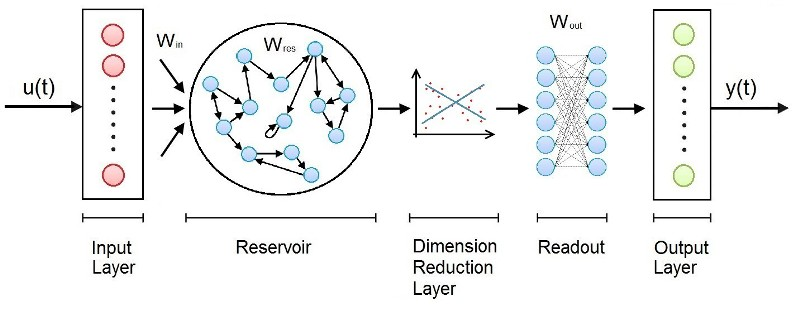
\includegraphics[width=\textwidth]{manuscript/src/figures/project/app3.jpeg}
    \end{minipage}
    \caption{Echo State Networks Architecture \cite{Bianchi2018ReservoirSeries}}
    \label{fig:a3}
\end{figure}